%% Beispiel-Präsentation mit LaTeX Beamer im KIT-Design
%% entsprechend den Gestaltungsrichtlinien vom 1. August 2020
%%
%% Siehe https://sdqweb.ipd.kit.edu/wiki/Dokumentvorlagen

%% Beispiel-Präsentation
\documentclass[en]{sdqbeamer} 

%% Footnote without numbering
\newcommand\nonumberfootnote[1]{%
  \begingroup
  \renewcommand\thefootnote{}\footnote{#1}%
  \addtocounter{footnote}{-1}%
  \endgroup
}
 
%% Titelbild
\titleimage{banner_2020_kit}

%% Gruppenlogo
\grouplogo{} 

%% Gruppenname und Breite (Standard: 50 mm)
\groupname{Institute for Automation and Applied Informatics (IAI)}
\groupnamewidth{60mm}

% Beginn der Präsentation

\title[ABAC for Substations]{Certificateless Attribute-Based Server-Aided Cryptosystem\\for Substation Automation Systems (CASC-SAS)}
\subtitle{Master's Thesis Presentation} 
\author[Moritz Gstuer]{Moritz Gstuer}
\date[12.\,12.\,2024]{12. December 2024}
% Literatur 
 
\usepackage[citestyle=authoryear,bibstyle=numeric,hyperref,backend=biber]{biblatex}
\addbibresource{../bibliography/masterthesis.bib}
\bibhang1em

\begin{document}
 
%Titelseite
\KITtitleframe

%Inhaltsverzeichnis
%\begin{frame}{Agenda}
%\tableofcontents
%\end{frame}

\section{Motivation}
\begin{frame}{Motivation}
    \begin{columns}
        \column{.55\textwidth}
        \centering
        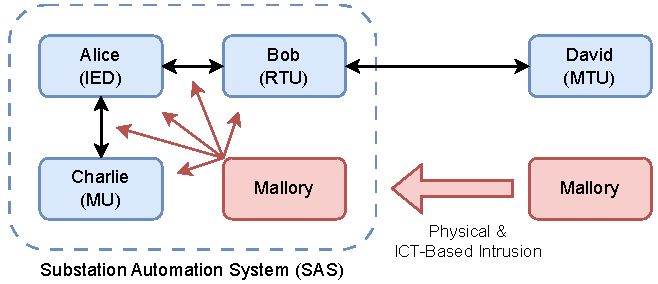
\includegraphics[width=1.0\textwidth]{./figures/sas_intrusion.drawio.pdf}
        \column{.45\textwidth}
        \begin{redblock}{Adversarial Attacks}
            \begin{itemize}
                \item \textbf{Availability-Focused:} Denial-of-Service\\$\rightarrow$ Malware, Flooding, \& Time-Delay
                \item \textbf{Integrity-Focused:} False Data Injection\\$\rightarrow$ Message Forgery, Modification, \& Replay
                \item \textbf{Authenticity-Focused:} Masquerading\\$\rightarrow$ Adaptive Chosen-Message, \& Collusion
            \end{itemize}
            % $\rightarrow$ Authentication, Authorization, Access Control, \& Encryption of Substation Communication
        \end{redblock}
    \end{columns}
    \nonumberfootnote{IED\dots Intelligent Electronic Device | MU\dots Merging Unit | RTU\dots Remote Terminal Unit}
    \nonumberfootnote{MTU\dots Master Terminal Unit | ICT\dots Information and Communications Technology}
\end{frame}
\begin{frame}{Research Questions}
    \begin{greenblock}{Authorization \& Access Control in SAS}
        How can expressive and flexible but yet computationally expensive access control be employed in a SAS?
        \\$\rightarrow$ Real-Time Attributes, Ad-Hoc Policy Evaluation, \& Speedup Solutions
    \end{greenblock}

    \begin{greenblock}{Public-Key Cryptography in SAS}
        How can a secure and lightweight public-key approach be designed, implemented, \& employed in a SAS?
        \\$\rightarrow$ (Dis-)Advantages, \& Speedup Solutions
    \end{greenblock}

    \begin{greenblock}{Security Architecture for Time-Critical Communication}
        How can authentication, authorization, and access control be integrated into a malleable, scalable, and lightweight cryptosystem for time-critical SAS communication?
        \\$\rightarrow$ System Model, Domain Requirements, Architecture, \& Protocols
    \end{greenblock}
\end{frame}

\section{Approach}
\begin{frame}{CASC-SAS Approach}
    \begin{greenblock}{\textbf{C}ertificateless \textbf{A}ttribute-Based \textbf{S}erver-Aided \textbf{C}ryptosystem for \textbf{S}ubstation \textbf{A}utomation \textbf{S}ystems (CASC-SAS)}
        Fine-grained \& flexible access control relying on dynamic authorization \& authentication
    \end{greenblock}
    \begin{blueblock}{\textbf{S}erver-Aided \textbf{A}ttribute-\textbf{B}ased \textbf{A}uthorization \& \textbf{A}ccess \textbf{C}ontrol (SABAAC)}
        Delegation of authorization \& access policy evaluation to semi-trusted server (PDP)
        \\$\rightarrow$ Enforcement of access control decisions via bump-in-the-wire device (PEP)
    \end{blueblock}
    \begin{blueblock}{\textbf{C}ertificateless \textbf{A}ttribute-Based \textbf{S}erver-Aided \textbf{A}uthentication (CASA)}
        Lightweight \& scalable algorithm-agnostic data frame authentication approach for deployment of PKC in SAS
        \\\textbf{Additionally:} $S_{CASA}$ $\rightarrow$ Certificateless attribute-based server-aided signature scheme
    \end{blueblock}
    \nonumberfootnote{PDP\dots Policy Decision Point | PEP\dots Policy Enforcement Point | PKC\dots Public Key Cryptography}
\end{frame}
\begin{frame}{CASC-SAS Architecture: Function-Oriented}
    \centering
    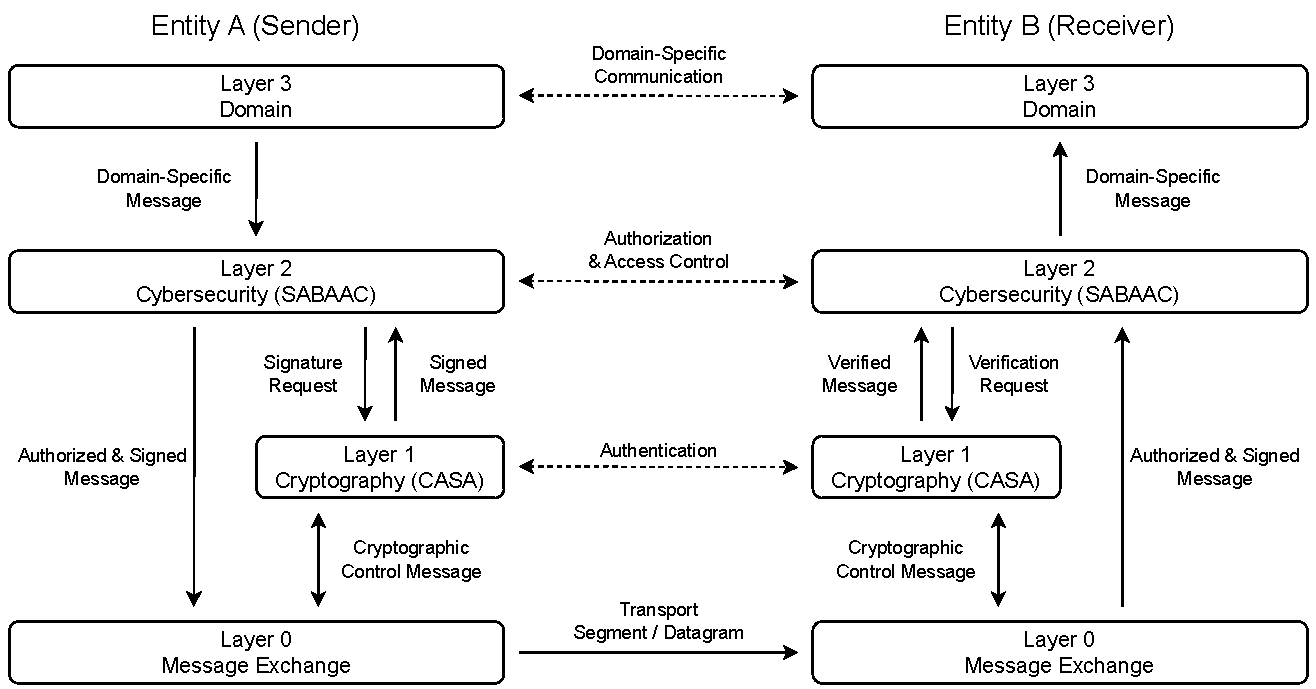
\includegraphics[height=0.75\textheight]{./figures/layers_request_example.drawio.pdf}
\end{frame}
\begin{frame}{CASC-SAS Architecture: Component-Oriented}
    \begin{columns}
        \column{.65\textwidth}
        \centering
        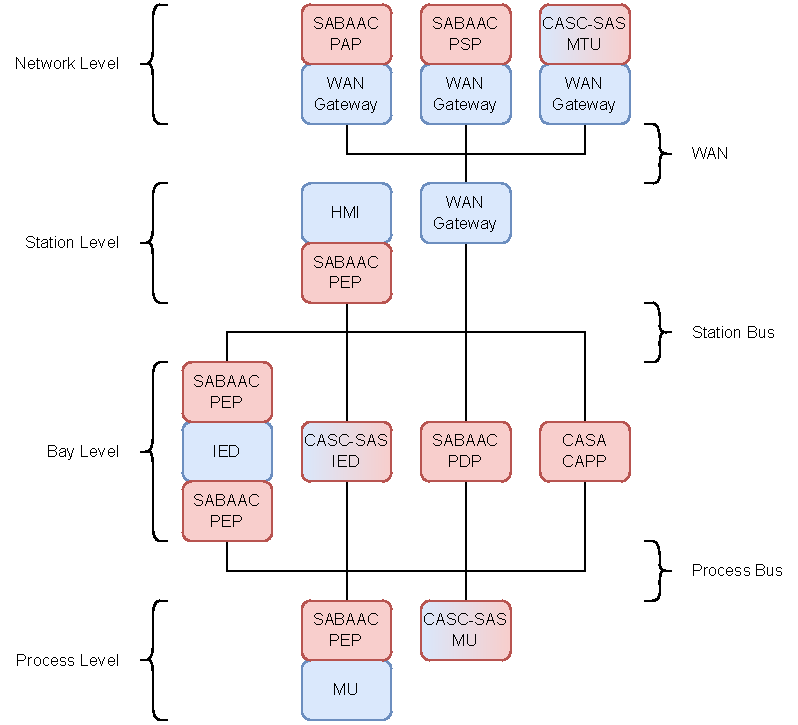
\includegraphics[height=0.75\textheight]{./figures/casc_architecture_color.drawio.pdf}
        \column{.35\textwidth}
        \footnotesize
        CAPP\dots CASA Administration\\\qquad\qquad\& Processing Platform\\HMI\dots Human-Machine Interface\\IED\dots Intelligent Electronic Device\\MTU\dots Master Terminal Unit\\MU\dots Merging Unit\\PAP\dots Policy Administration Point\\PDP\dots Policy Decision Point\\PEP\dots Policy Enforcement Point\\PSP\dots Policy Storage Point\\RTU\dots Remote Terminal Unit\\WAN\dots Wide Area Network
    \end{columns}
\end{frame}
\begin{frame}{Performance Analysis (Preliminary): UDP Echo}
    \begin{columns}
        \column{.46\textwidth}
        \begin{blueblock}{Access Control Overhead}
            \begin{tabular}{r r r r}
                & \multicolumn{1}{c}{Avg} & \multicolumn{1}{c}{Min} & \multicolumn{1}{c}{Throughput}\\
                \textbf{Unauthorized} & 2.0 ms & 1.7 ms & 465 PPS\\
                \textbf{Unsigned} & 3.3 ms & 2.8 ms & 292 PPS
            \end{tabular}
            %\textbf{Unauthorized:} $\sim$2.0 ms RTT (min $\sim$1.7 ms) 465 PPS
            %\\\textbf{Unsigned:} $\sim$3.3 ms RTT (min $\sim$2.8 ms) 292 PPS
            %\vspace{0.1em}
            \\$\rightarrow$ Access Control: +1.3 ms RTT (+65 \%)
        \end{blueblock}
        \begin{blueblock}{Authentication Overhead}
            \begin{tabular}{r r r r}
                & \multicolumn{1}{c}{Avg} & \multicolumn{1}{c}{Min} & \multicolumn{1}{c}{Throughput}\\
                \textbf{HMAC} & 3.4 ms & 2.9 ms & 285 PPS\\
                \textbf{Ed25519} & 12.0 ms & 9.6 ms & 82 PPS\\
                \textbf{RSA-2048} & 14.0 ms & 11.4 ms & 68 PPS
            \end{tabular}
            %\textbf{HMAC:} $\sim$3.4 ms RTT (min $\sim$2.9 ms) 285 PPS
            %\\\textbf{Ed25519:} $\sim$12.0 ms RTT (min $\sim$9.6 ms) 82 PPS
            %\\\textbf{RSA-2048:} $\sim$14.0 ms RTT (min $\sim$11.4 ms) 68 PPS
            %\vspace{0.1em}
            \\$\rightarrow$ Authentication: +0.1--10.7 ms RTT (+3--325 \%)
        \end{blueblock}
        \column{.54\textwidth}
        \centering
        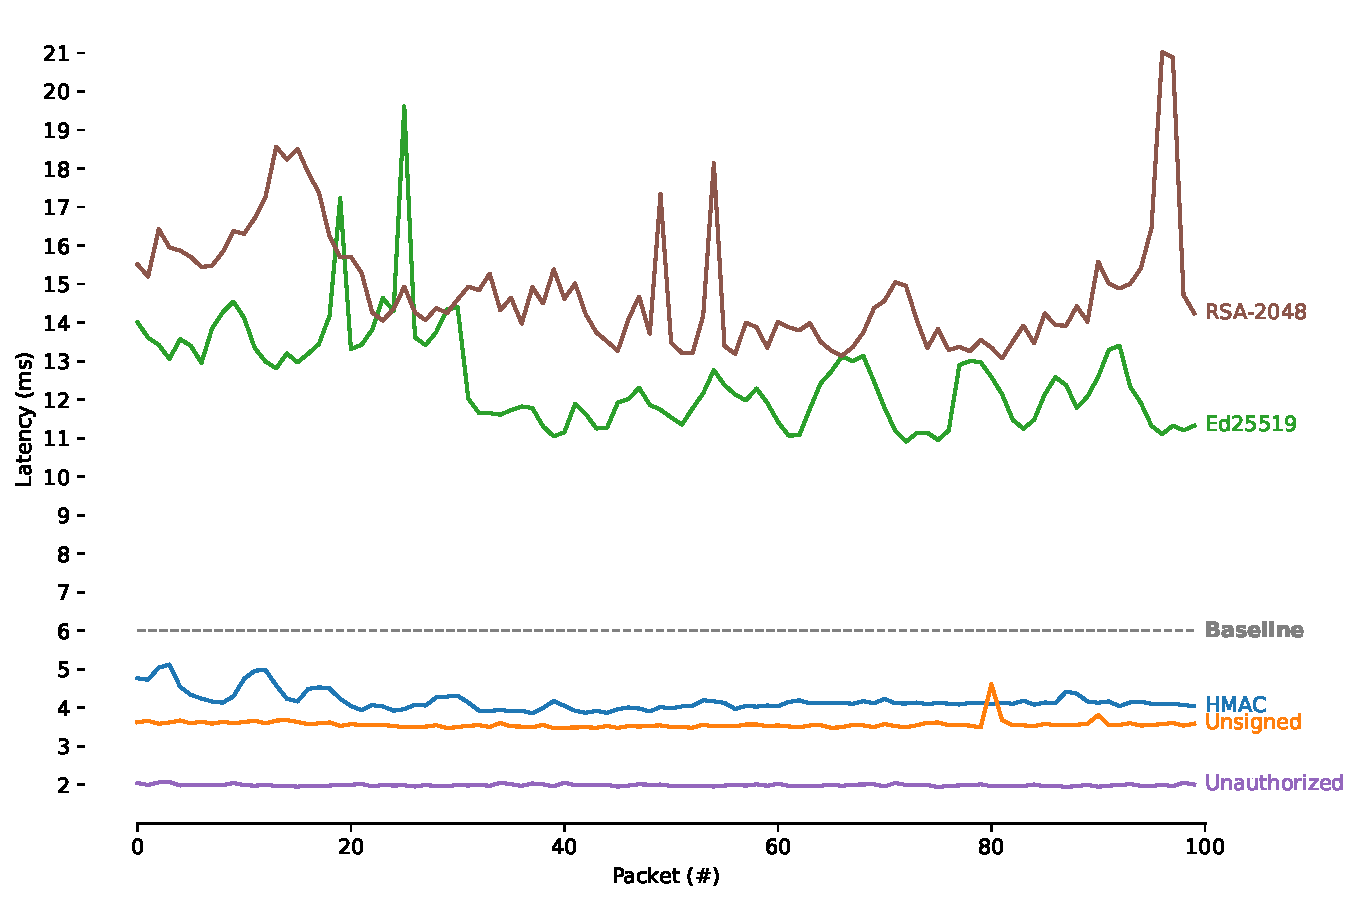
\includegraphics[height=0.72\textheight]{./figures/rtt-estimation-results.pdf}
    \end{columns}
    \nonumberfootnote{RTT\dots Round-Trip Time | PPS\dots Packets Per Second (Sequential) | Baseline\dots 6 ms (3 ms Request \& 3 ms Response)}
\end{frame}

\section{Future Work}
\begin{frame}{Future Work I}
    \begin{blueblock}{Cryptography-Driven Authentication, Authorization, \& Access Control}
        Authentication, authorization, \& access control in a single attribute-based PKC scheme
        \\$\rightarrow$\textbf{Advantage:} Privacy \& Anonymity
    \end{blueblock}
    \begin{blueblock}{Encryption \& Decryption}
        Encryption \& decryption in conjunction with signing \& verification operations
        \\$\rightarrow$\textbf{Advantage:} Confidentiality
    \end{blueblock}
    \begin{blueblock}{Hardware Acceleration}
        Advantages \& disadvantages of hardware-based cryptography acceleration in SAS
        \\$\rightarrow$\textbf{Advantage:} Decreased computation time \& increased message throughput
        \\$\rightarrow$\textbf{Risk:} Algorithm compatibility, costs per acceleration unit, \& computation time consistency
    \end{blueblock}
\end{frame}
\begin{frame}{Future Work II}
    \begin{blueblock}{AI for Policy Management}
        Linking of CASC-SAS with AI-based intrusion detection for the creation and modification of security policies
        \\$\rightarrow$\textbf{Advantage:} Mitigation of a wider range of cyberattacks in a timelier manner
    \end{blueblock}
    \begin{blueblock}{SDN-Based Approach Realization}
        Aggregation of multiple PEPs by deploying a virtual PEP for each port of a Software-Defined Networking (SDN) switch.
        \\$\rightarrow$\textbf{Advantage:} Reduced costs of deployment \& reduced architectural complexity
    \end{blueblock}
\end{frame}

\section{Conclusion}
\begin{frame}{Conclusion}
    \begin{redblock}{Problem}
        Expressive \& flexible access control, \& malleable PKC: Not applicable to the SAS domain!
        \\$\rightarrow$ Constrained resource \& communication time
    \end{redblock}
    \begin{blueblock}{Contribution}
        CASC-SAS security architecture \& framework\dots
        \\\dots employs mandatory authentication, authorization, \& access control
        \\\dots for time-critical SAS communication
        \\\dots in time-variable SAS environment.
    \end{blueblock}
    \vspace{0.5em}
    \centering
    \huge
    Thank you!
\end{frame}

\appendix
\beginbackup
\begin{frame}{~}
    \centering
    \huge
    Appendix
\end{frame}
\section{System Model}
\begin{frame}{Motivation}
    \centering
	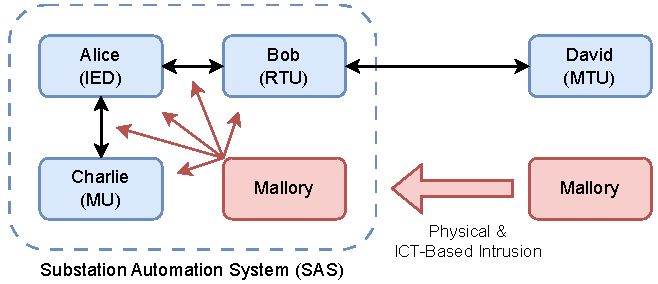
\includegraphics[width=0.8\textwidth]{./figures/sas_intrusion.drawio.pdf}
    \nonumberfootnote{IED\dots Intelligent Electronic Device | MU\dots Merging Unit | RTU\dots Remote Terminal Unit}
    \nonumberfootnote{MTU\dots Master Terminal Unit | ICT\dots Information and Communications Technology}
\end{frame}
\begin{frame}{System Model: Substation Automation System (SAS)}
    \centering
    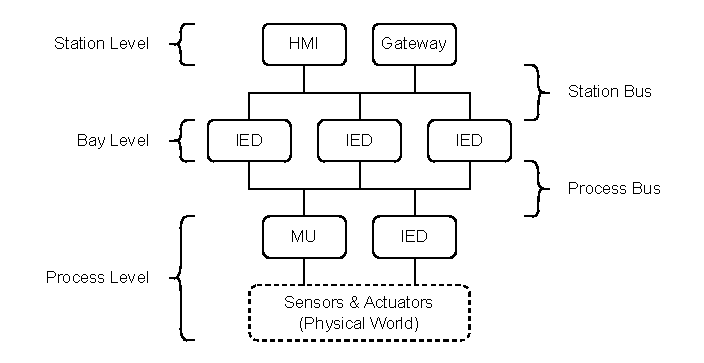
\includegraphics[width=0.7\textwidth]{./figures/substation_architecture.drawio.pdf}
    \nonumberfootnote{IED\dots Intelligent Electronic Device | MU\dots Merging Unit | HMI\dots Human-Machine Interface}
\end{frame}
\begin{frame}{SAS Communication: Requirements \& Constraints}
    \begin{blueblock}{Requirements}
        \begin{itemize}
            \item Integrity
            \item Authenticity
            \item Non-Repudiation
            \item Least Privilege Principle (PoLP)
            \item Separation of Duties (SoD)
        \end{itemize}
        $\rightarrow$ Authentication, Authorization, \& Access Control
    \end{blueblock}
    \begin{grayblock}{Constraints: IEC 61850 Message Types \& Performance Classes \parencite*{IEC61850P5,IEC61850P8}}
        Client-Server (Unicast) \& Publisher-Subscriber (Broadcast/Multicast) \\$\rightarrow$ Resource \& Time Constraints!
        \\Examples: GOOSE (Type 1A, 3 ms), SV (Type 4, 3 ms), MMS (Type 2/3/5, 100-10000 ms)
    \end{grayblock}
\end{frame}

\section{Related Work}
\begin{frame}{Related Work}
    \begin{blueblock}{IEC 62351 \parencite*{IEC62351P6,IEC62351P8}}
        Standard for Cybersecurity: Energy-Related Systems \& Communication Networks
        \\$\rightarrow$ Authenticity \& Integrity: Mandatory Symmetric Authentication
        \\$\rightarrow$ Confidentiality: Optional (Non-Recommended) Symmetric Encryption
        \\$\rightarrow$ Access Control: Role-Based Access Control (RBAC) (Access-Token-Driven, 7 Mandatory Roles)
    \end{blueblock}
\end{frame}
\begin{frame}{Related Work}
    \begin{blueblock}{Secure Communication in Substations}
        \begin{itemize}
            \item Bump-in-the-Wire Security Filter for GOOSE/SV MAC Tagging \& Verification \parencite{Ishchenko2018}
            \item Domain-Based Collaborative Cyberattack Mitigation Approach \parencite{Hong2019}
            \item Fixed-Latency Hardware Architecture for GOOSE/SV Encryption \& Authentication \parencite{Rodriguez2021}
        \end{itemize}
    \end{blueblock}

    \begin{blueblock}{Role-Based Access Control (RBAC) in Substations}
        \begin{itemize}
            \item XACML-Based RBAC Approach for IEC 61850 \& IEC 62351 compliant SAS \parencite{Lee2015}
            \item Distributed RBAC for Subscription-Based Remote Network Services \parencite{Ma2006} % Constraint-Enabled 
            \item Rule-Based RBAC Policy Enforcement Architecture \parencite{Alcaraz2016} % for Smart Grid Systems
        \end{itemize}
    \end{blueblock}
\end{frame}
\begin{frame}{Related Work}
    \begin{blueblock}{Attribute-Based Access Control (ABAC) in Substations}
        \begin{itemize}
            \item Firewall for Attribute-Based Access Control in Smart Grids \parencite{Ruland2018}
            \\$\rightarrow$ Firewall with XACML-Based ABAC Policies
            \\$\rightarrow$ Outer \& Inner Station Bus
            \\$\rightarrow$ Unobstructed Fast Messages (e.g. GOOSE)
            \item T-ABAC: An attribute-based access control model for real-time availability in highly dynamic systems \parencite{Burmester2013}
            \\$\rightarrow$ Real-Time Attribute Values
            \\$\rightarrow$ Labeling of High Priority Packets
            \\$\rightarrow$ Domain-Based Congestion Avoidance
        \end{itemize}
    \end{blueblock}
    % Message Authentication, Asym. Performance Evaluation, BitW- \& HW-Solutions, Access Control
\end{frame}

\section{Access Control}
\begin{frame}{Traditional Authorization, Authentication, \& Access Control}
    \centering
	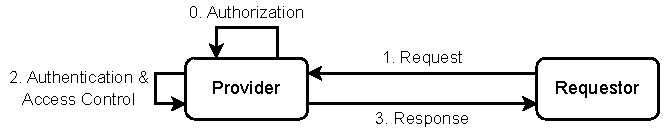
\includegraphics[width=0.9\textwidth]{./figures/access_control_request_traditional.drawio.pdf}
    \begin{redblock}{Problem}
        Too many provider responsibilities
        \\$\rightarrow$ Policy Management/Decisions/Enforcement, Request Verification, \& Response Creation
    \end{redblock}
\end{frame}
\begin{frame}{Attribute-Based Access Control (ABAC)}
    \begin{greenblock}{Definition \parencite{JTF2020}}
        Access control model enabling access decisions based on attributes associated with \textbf{subjects}, \textbf{objects}, \textbf{actions}, and the \textbf{environment} of a system.
    \end{greenblock}

    \begin{blueblock}{Discussion \parencite{Hu2014}}
        \begin{itemize}
            \item Multifactor Policy Expression $\rightarrow$ Fine-Grained \& Flexible Access Control (cf. RBAC/IBAC)
            \item Dynamic Policy Evaluation $\rightarrow$ Dynamic Authorization \& Real-Time Attributes
        \end{itemize}
    \end{blueblock}

    \begin{grayblock}{Architecture \parencite{Hu2014,Oasis2013}}
        \begin{itemize}
            \item Policy Decision Point (PDP) $\rightarrow$ Computes access decisions by evaluating policies
            \item Policy Enforcement Point (PEP) $\rightarrow$ Enforces policy decisions by controlling access to protected objects
        \end{itemize}
    \end{grayblock}
    % ABAC Definition
    % ABAC Benefit vs. traditional IBAC/RBAC solutions including RT-Attribute like network congestion
    % ABAC Requirements -> Authentication \& Authorization
\end{frame}
\begin{frame}{Server-Aided ABAC}
    \centering
    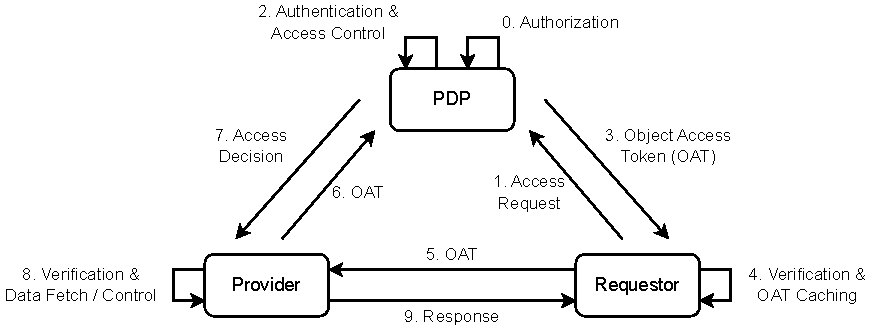
\includegraphics[width=1.0\textwidth]{./figures/access_control_request_delegation.drawio.pdf}
\end{frame}
\begin{frame}{CASC-SAS: Authentication, Authorization, \& Access Control}
    \begin{redblock}{Problem: Policy Evaluation Complexity}
        Fine-grained \& flexible access control relying on dynamic authorization \& authentication
        \\$\rightarrow$ Ad-hoc evaluation in real-time environment
    \end{redblock}

    \begin{greenblock}{Solution: Server-Aided Access Control}
        Delegation of authorization \& access control to semi-trusted server (PDP)
        \\$\rightarrow$ Authentication at each device (server-aided)
        \\$\rightarrow$ Speedup Techniques: Evaluation pre-computation \& access decision caching
    \end{greenblock}

    \begin{grayblock}{Architecture \parencite{Hu2014,Oasis2013}}
        \begin{itemize}
            \item Policy Decision Point (PDP) $\rightarrow$ Computes access decisions by evaluating policies
            \item Policy Enforcement Point (PEP) $\rightarrow$ Enforces policy decisions by controlling access to protected objects
        \end{itemize}
    \end{grayblock}
\end{frame}

\section{Evaluation}
\begin{frame}{Performance Evaluation}
    \begin{greenblock}{Question}
        Is CASC-SAS capable of securing time-constrained communication of a SAS?
        \\$\rightarrow$ Computational complexity, supported message types, \& network exception resilience
    \end{greenblock}
    \begin{blueblock}{Approach}
        Experimentally performed evaluation based on realization
        \\$\rightarrow$ Currently: Testbed-based experiments
        \\$\rightarrow$ Planned: Lab-based experiments
    \end{blueblock}
\end{frame}

\begin{frame}[allowframebreaks]{References}
\printbibliography
\end{frame}

\backupend

\end{document}